\label{sec:cicd}

Aktuell läuft das Deployment von LearnHub manuell. Bei jeder 
Code-Änderung werden die Docker-Images von Hand gebaut, auf Docker 
Hub hochgeladen und auf der VM neu gestartet. Das funktioniert für 
den aktuellen Projektumfang, ist aber auf Dauer fehleranfällig und 
zeitaufwendig. Eine vollständige CI/CD-Pipeline würde diesen Prozess 
automatisieren \cite{fowler2006continuous}.

\subsubsection{GitHub Actions}

Für LearnHub wurde \textbf{GitHub Actions} eingesetzt, da der Code 
bereits auf GitHub liegt und GitHub Actions direkt integriert ist. 
Ein Workflow wird in einer YAML-Datei unter 
\texttt{.github/workflows/} definiert und von GitHub automatisch 
ausgeführt wenn ein bestimmtes Ereignis eintritt.

Abbildung~\ref{fig:github-actions-workflow} zeigt den aktuellen 
Workflow für das Backend von LearnHub.

\begin{figure}[H]
    \centering
    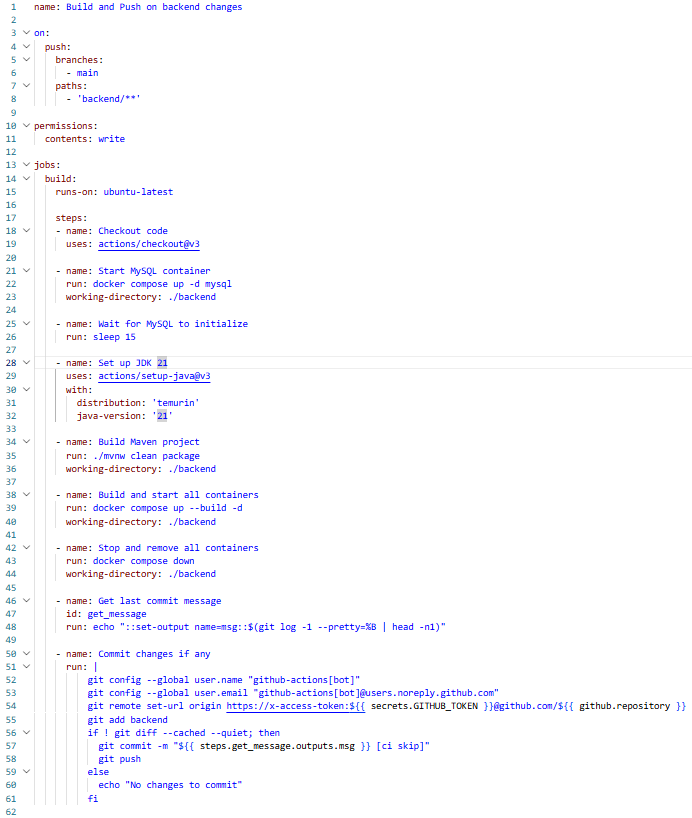
\includegraphics[width=\textwidth]{pics/github_actions_workflow.png}
    \caption{GitHub Actions Workflow für das Backend}
    \label{fig:github-actions-workflow}
\end{figure}

\subsubsection{Aufbau des Workflows}

Der Workflow wird automatisch ausgelöst wenn Code im 
\texttt{backend} Verzeichnis auf den Main-Branch gepusht wird. 
Er besteht aus einem einzigen Job der folgende Schritte ausführt:

Zuerst wird ein MySQL Container gestartet da der Maven Build 
eine laufende Datenbank benötigt. Nach einer kurzen Wartezeit 
bis MySQL bereit ist, wird JDK 21 eingerichtet und das Backend 
mit \texttt{mvn clean package} gebaut. Danach werden alle 
Container gebaut und gestartet um zu prüfen ob alles 
zusammenspielt, anschließend wieder gestoppt.

Zum Schluss prüft der Workflow ob der Build Änderungen im 
\texttt{backend} Verzeichnis erzeugt hat. Falls ja, werden 
diese automatisch committed und mit der ursprünglichen 
Commit-Message zurück ins Repository gepusht. Der Commit 
enthält den Zusatz \texttt{[ci skip]} damit er nicht 
erneut den Workflow auslöst.

Sensible Informationen wie der GitHub Token werden als 
\textbf{GitHub Secrets} gespeichert und im Workflow über 
\texttt{\$\{\{ secrets.GITHUB\_TOKEN \}\}} referenziert, 
sodass sie nie im Quellcode stehen \cite{github_secrets}.

Abbildung~\ref{fig:cicd-pipeline} zeigt den Ablauf des 
Workflows als Diagramm.

\begin{figure}[H]
    \centering
    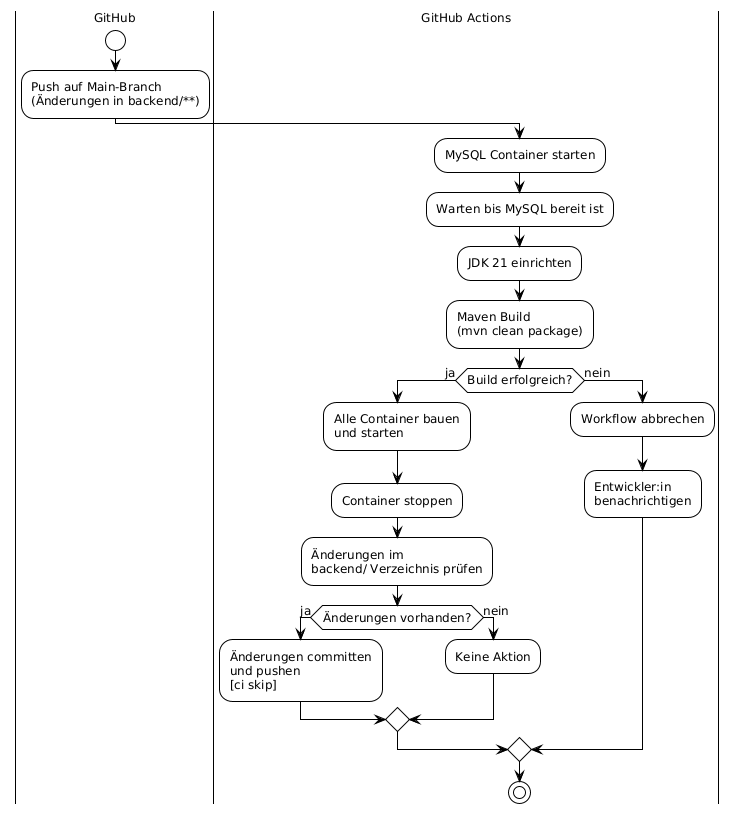
\includegraphics[width=0.75\textwidth]{pics/ci_cd.png}
    \caption{Ablauf der CI/CD Pipeline}
    \label{fig:cicd-pipeline}
\end{figure}

Wie in Abbildung~\ref{fig:cicd-pipeline} zu sehen, wird der 
Workflow nur ausgelöst wenn Änderungen im \texttt{backend} 
Verzeichnis auf den Main-Branch gepusht werden. Der Build 
benötigt eine laufende MySQL Datenbank, weshalb zuerst ein 
MySQL Container gestartet wird. Schlägt der Maven Build fehl, 
bricht der Workflow ab und die Entwickler:in wird 
benachrichtigt. Bei Erfolg werden alle Container kurz gestartet 
um das Zusammenspiel zu prüfen, dann wieder gestoppt. Falls 
der Build Änderungen erzeugt hat, werden diese automatisch 
zurück ins Repository gepusht.

Ein Frontend-Workflow sowie ein automatisches Deployment 
auf die VM sind aktuell noch nicht implementiert und wären 
ein sinnvoller nächster Schritt für die Weiterentwicklung 
der Pipeline.

\subsubsection{Automatisierte Tests}

Der aktuelle Workflow führt den Maven Build mit 
\texttt{mvn clean package} aus, wobei auch die vorhandenen 
Backend-Tests ausgeführt werden. Für eine vollständigere 
Teststrategie eignen sich zusätzlich Integration-Tests mit 
\texttt{@QuarkusTest}, womit HTTP-Requests simuliert werden 
können \cite{quarkus-testing}. Für Datenbank-Tests kann eine 
In-Memory H2-Datenbank verwendet werden um unabhängig von der 
produktiven MySQL-Datenbank zu bleiben.

Für das Angular-Frontend sind aktuell keine automatisierten 
Tests in der Pipeline implementiert. Sinnvoll wären 
Unit-Tests mit Jasmine und Karma sowie End-to-End-Tests 
mit Cypress oder Playwright \cite{cypress-docs}.

\subsubsection{Rollback}

Da der Quellcode versioniert auf GitHub liegt, ist ein Rollback 
jederzeit möglich indem ein früherer Commit ausgecheckt und neu 
gebaut wird. Für eine vollständige Pipeline wäre zusätzlich das 
Taggen von Docker-Images mit der Versionsnummer sinnvoll, sodass 
auch auf der VM direkt auf eine frühere Image-Version 
zurückgewechselt werden kann.